\section{Introduction}

% Guttel: Matrix functions are interesting for scientific computing because they arise in explicit so- lution formulas for relevant algebraic and differential equations.
\todo{Add motivation and applications (exponential integrators, etc.)}

\newpage
\section{Matrix Functions}

\subsection{Univariate Matrix Functions}
This section reviews the basic definition and properties of matrix functions
discussed in detail in \cite{higham2008functions}.
Let $A \in \mathbb{C}^{n \times n}$ have $s$ distinct eigenvalues $\Lambda(A) = \{\lambda_k\}_{k=1}^{s}$.
$A$ can be expressed in the Jordan canonical form as $A = ZJZ^{-1} = Z \diag(J_k)_{k=1}^{s}
Z^{-1}$. Let $m_k$ denote the size of the largest Jordan block associated
with $\lambda_k$. The matrix function associated with a univariate function $f$
is defined by $f(A) := g(A)$, where $g(z)$ is the unique Hermite interpolating
polynomial of degree less than $\sum_{k=1}^{s}{m_k}$, which satisfies
\begin{equation}
    \frac{\partial^j}{\partial z^j}g(\lambda_k) = \frac{\partial^j}{\partial z^j}f(\lambda_k),
    \quad \forall j \in \{0, 1, \dots, m_k-1\},
    \quad \forall k \in \{1, 2, \dots, s\},
\end{equation}
assuming that all required derivatives of $f(z)$ exist.

Equivalently, $f(A)$ could also be defined as $f(A) := Z \diag(f(J_k))_{k=1}^{s} Z^{-1}$ where
\begin{equation*}
    f(J_k) =
    \begin{bmatrix}
    f(\lambda_k) & f'(\lambda_k)  & \frac{1}{2} f^{(2)}(\lambda_k) & \cdots & \frac{f^{(m_k-1)}(\lambda_k)}{(m_k - 1)!}\\
    & f(\lambda_k) & f'(\lambda_k) & \cdots & \frac{f^{(m_k-2)}(\lambda_k)}{(m_k - 2)!} \\
    &  & f(\lambda_k) & \ddots & \vdots \\
    &  &  & \ddots & f'(\lambda_k)\\
    &  &  &  & f(\lambda_k)
    \end{bmatrix}.
\end{equation*}

If $A = Z \diag(\lambda_k)_{k=1}^{n} Z^{-1}$ is diagonalizable, we have
\begin{equation}
    \label{eq:matrixfunctiondiagonal}
    f(A) = Z \diag(f(\lambda_k))_{k=1}^{n} Z^{-1}.
\end{equation}

A third equivalent definition is via Cauchy integral and it reads
\begin{equation}
    f(A) := \frac{1}{2 \pi i} \int_{\Gamma}{f(z)(zI - A)^{-1} dz},
\end{equation}
assuming that $f$ is analytic on and inside a closed contour $\Gamma$ that encloses $\Lambda(A)$.

\subsection{Matrix Exponential}
The matrix function attributed to the scalar exponential function is called
matrix exponential and is defined~\cite{higham2008functions} as
\begin{equation}
    \label{eq:matrixexponentialdefinition}
    \exp(A) = \sum_{k=0}^{\infty}{\frac{1}{k!} A^k}.
\end{equation}

Some properties of the matrix exponential follows:
\begin{itemize}
    \item By taking the conjugate transpose of \eqref{eq:matrixexponentialdefinition},
        we can conclude $\exp(A^{*}) = \exp(A)^{*}$.
    \item For every $B \in \mathbb{C}^{n \times n}$ that satisfies $AB = BA$,
        we have $\exp(A + B) = \exp(A) \exp(B)$.
    \item $\exp(A)$ is always invertible and its inverse is $\exp(A)^{-1} = \exp(-A)$.
    \item The derivative of $\exp(tA)$ with respect to a scalar $t$ is given by
        $\frac{\mathrm{d}}{\mathrm{d} t} (\exp(tA)) = A \exp(tA)$.
    \item The determinant of $\exp(A)$ is the exponential of the trace of
        $A$: $\det(\exp(A)) = \exp(\trace(A))$.
\end{itemize}

\begin{figure}[h]
    \centering
    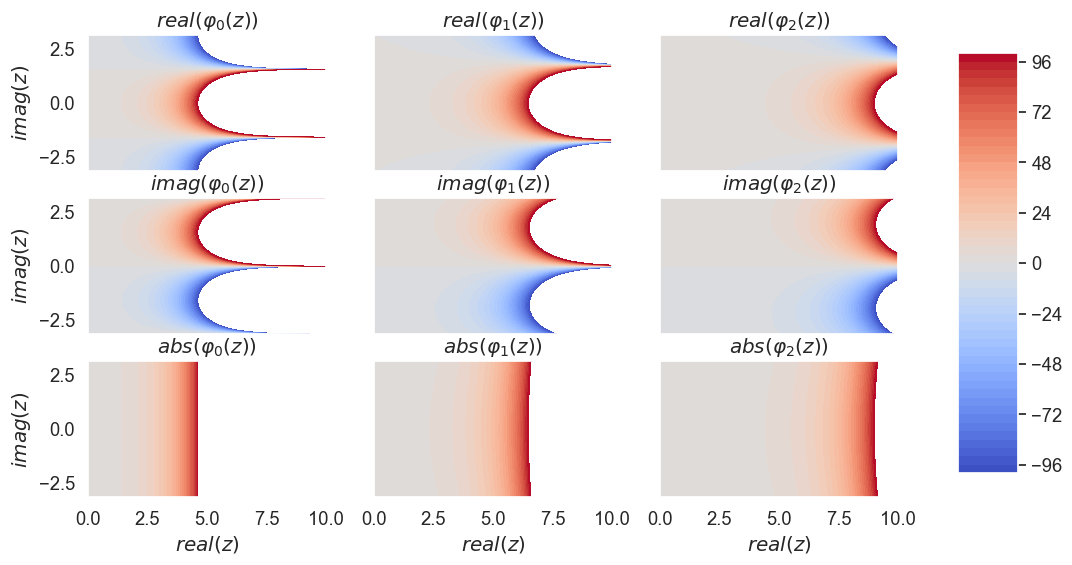
\includegraphics[width=.7\textwidth]{img/scalarcomplexplane.png}
    \caption{
        Evaluation of scalar $\varphi$-functions on the complex plane.
        The values that are out of the range of the color bar are not visualized.
        }
    \label{fig:scalarphifunctionscomplexplane}
\end{figure}


\subsection{\texorpdfstring{$\varphi$}{Phi}-functions}
\todo[color=cyan]{Add applications and motivation.}
There is a class of matrix functions called $\varphi$-functions that are essential
for exponential integrators for ordinary differential equations. Accurate and efficient
evaluation of these functions is necessary for implementation of exponential integrators.
For a scalar argument $z \in \mathbb{C}$, they are defined~\cite{higham2008functions} as
\begin{equation}
    \label{eq:scalarphifunctionsdefinition}
    \varphi_0(z) = \exp(z), \qquad
    \varphi_p(z) = \frac{1}{(p-1)!} \int_{0}^{1}{e^{(1 - \theta)z} \theta^{p-1} d\theta},
    \quad p \in \mathbb{N^*}.
\end{equation}

The $\varphi$-functions satisfy~\cite{higham2008functions} the recurrence relation
\begin{equation}
    \label{eq:scalarphifunctionsrecurrence}
    \varphi_p(z) = z^{-1} \left[ \varphi_{p-1}(z) - \frac{1}{(p-1)!} \right] ,
    \quad z \neq 0, \quad p \in \mathbb{N^*},
\end{equation}
and $\varphi_p(z) = \frac{1}{p!}$ for $z=0$.

The evaluation of the first three scalar $\varphi$-functions on the left half complex plane
is illustrated in \autoref{fig:scalarphifunctionscomplexplane}. Note that the gradients are
smaller for higher $p$'s.


We can use \eqref{eq:scalarphifunctionsrecurrence} recursively as
\begin{equation*}
    \begin{aligned}
        \varphi_p(z) & = z^{-1} \varphi_{p-1}(z) - \frac{1}{(p-1)!} z^{-1} \\
        & = z^{-1} \left[ z^{-1} \varphi_{p-2}(z) - \frac{1}{(p-2)!} z^{-1} \right] - \frac{1}{(p-1)!} z^{-1} \\
        & = z^{-2} \varphi_{p-2}(z) - \frac{1}{(p-2)!} z^{-2} - \frac{1}{(p-1)!} z^{-1} \\
        & = \cdots \\
        & = z^{-p} \varphi_{0}(z) - \frac{1}{0!} z^{-p} - \frac{1}{1!} z^{-(p-1)} - \frac{1}{2!} z^{-(p-2)} - \cdots - \frac{1}{(p-1)!} z^{-1} \\
        & = z^{-p} \exp(z) - \sum_{k=0}^{p-1}{\frac{1}{k!}z^{-(p-k)}}
        \end{aligned}
\end{equation*}
to derive a closed form for $\varphi_p$:
\begin{equation}
    \label{eq:scalarphifunctionsclosedform}
    \varphi_p(z) = z^{-p} \left( \exp(z) - \sum_{k=0}^{p-1}{\frac{1}{k!}z^{k}} \right), \quad z \neq 0.
\end{equation}

% CHECK: What if A is singular?
For an invertible matrix $A \in \mathbb{C}^{n \times n}$, we can do the same steps
and use \eqref{eq:matrixexponentialdefinition} to get
\begin{equation}
    \label{eq:matrixphifunctionsclosedform}
    \varphi_p(A) = A^{-p} \left( \exp(A) - \sum_{k=0}^{p-1}{\frac{1}{k!}A^{k}} \right)
    = \sum_{k=0}^{\infty}{\frac{1}{(k+p)!} A^{k}}.
\end{equation}

\subsection{Trigonometric Matrix Functions}
\label{sec:trigonometricmatrixfunctions}

The two most important trigonometric functions, sine and cosine, are defined
\cite{higham2008functions} for all $A \in \mathbb{C}^{n \times n}$ by
\begin{equation}
    \label{eq:matrixcosinedefinition}
    \cos(A) = I - \frac{A^2}{2!} + \frac{A^4}{4!} - \frac{A^6}{6!} + \cdots
    = I + \sum_{k=1}^{\infty}{\frac{(-1)^k}{(2k)!} A^{2k}};
\end{equation}
and
\begin{equation}
    \label{eq:matrixsinedefinition}
    \sin(A) = A - \frac{A^3}{3!} + \frac{A^5}{5!} - \frac{A^7}{7!} + \cdots
    = A + \sum_{k=1}^{\infty}{\frac{(-1)^k}{(2k+1)!} A^{2k+1}}.
\end{equation}
The matrix sinc function associated with the scalar sinc function
$\mathrm{sinc}(z) = \sin(z) / z$ is defined by
\begin{equation}
    \label{eq:matrixsincdefinition}
    \begin{aligned}
        \mathrm{sinc}(A) & = A^{-1} \sin(A)
        = I - \frac{A^2}{3!} + \frac{A^4}{5!} - \frac{A^6}{7!} + \cdots \\
        & = I + \sum_{k=1}^{\infty}{\frac{(-1)^k}{(2k+1)!} A^{2k}}.
    \end{aligned}
\end{equation}
Some properties of the matrix sine and cosine follows:
\begin{itemize}
    \item The matrix analoge of Euler's formula reads $e^{iA} = \cos(A) + i \sin(A)$.
    \item For all $A \in \mathbb{C}^{n \times n}$ we have $\cos(A) = \frac{1}{2} (e^{iA} + e^{-iA})$.
    \item For all $A \in \mathbb{C}^{n \times n}$ we have $\sin(A) = \frac{1}{2i} (e^{iA} - e^{-iA})$.
    \item For all $A \in \mathbb{C}^{n \times n}$ we have $\cos^2(A) + \sin^2(A) = I$.
    \item For real $A \in \mathbb{R}^{n \times n}$ we have $\cos(A) = \mathfrak{Re}(e^{iA})$.
    \item For real $A \in \mathbb{R}^{n \times n}$ we have $\sin(A) = \mathfrak{Im}(e^{iA})$.
\end{itemize}

\begin{comment}
\subsection{Bivariate Matrix Functions}
Let $A \in \mathbb{C}^{n \times n}$ have $s$ distinct eigenvalues $\{\lambda_i\}_{i=1}^{s}$
and $B \in \mathbb{C}^{m \times m}$ have $t$ distinct eigenvalues $\{\mu_i\}_{i=1}^{t}$.
Consider a bivariate polynomial $p(x, y) = \sum_{i=1}^{s} \sum_{j=1}^{t} p_{ij} x^i y^j$
with $p_{ij} \in \mathbb{C}$. Then $p\{A, B\}: \mathbb{C}^{m \times n} \to \mathbb{C}^{m \times n}$
is defined~\cite{kressner2014bivariate} by
\begin{equation}
    \sum_{i=1}^{s} \sum_{j=1}^{t} p_{ij} A^i C (B^\top)^j.
\end{equation}

The bivariate matrix function associated with a general bivariate scalar function
$f(x, y)$ is a linear operator on $\mathbb{C}^{n \times m}$ and is
defined~\cite{kressner2014bivariate} by $f\{A, B\} := p\{A, B\}$, where $p$ is the
unique Hermite interpolating polynomial which satisfies
\begin{equation*}
    \frac{\partial^{g+h}}{\partial^g x \partial^h y}p(\lambda_i, \mu_j)
    = \frac{\partial^{g+h}}{\partial^g x \partial^h y}f(\lambda_i, \mu_j),
    \quad
    \begin{matrix}
        \forall g \in \{0, 1, \dots, ind_{\lambda_i(A)}-1\},
        & \forall i \in \{1, 2, \dots, s\},
        \\
        \forall h \in \{0, 1, \dots, ind_{\mu_j(B)}-1\},
        & \forall j \in \{1, 2, \dots, t\}.
    \end{matrix}
\end{equation*}
$f$ only exists if the mixed partial derivatives in the definition exist and
are continuous.
\end{comment}

\newpage
\section{Methodology}\label{sec:methods}

\subsection{Krylov Subspaces and the Arnoldi Algorithm}\label{sec:arnoldi}
Given a matrix $A \in \mathbb{C}^{n \times n}$ and a vector $v \neq 0 \in \mathbb{C}^n$,
the Krylov subspace of order $m \leq n$ for them is defined \cite{golub2013matrix} as
\begin{equation}
    \label{eq:krylovsubspacedefinition}
    \begin{aligned}
        \mathcal{K}_m(A, v) & := \setspan\{v, Av, A^{2}v, \dots, A^{m-1}v \}\\
         & = \{g(A)v \:|\: g \in \Pi_{m-1} \},
    \end{aligned}
\end{equation}
where $\Pi_{m-1}$ is the set of all polynomials of order up to $m-1$.
Krylov supspaces are essential in many methods in numerical linear algebra
for solving eigenvalue problems. However, the vectors $v, Av, A^{2}v, \dots, A^{m-1}v$
are not a good basis for $\mathcal{K}_m(A, v)$. We know from the power method that
these vectors have almost the same direction and converge to the eigenvector paired
with the biggest eigenvalue of $A$.
From the Arnoldi algorithm \cite{trefethen1997numerical} described in Algorithm
\ref{alg:polynomialarnoldi}, we can get an orthonormal basis for $\mathcal{K}_m(A, v)$
and an upper Hessenberg matrix $H_m = V_m^* A V_m$. The Arnoldi factorization reads
\begin{equation}
    \label{eq:arnoldifactorization}
    A V_m = V_m H_m + h_{m+1, m} v_{m+1} e_m^\top,
\end{equation}
where $e_m$ is the last canonical basis vector of $\mathbb{R}^{m}$.

\begin{algorithm}
    \caption{Arnoldi algorithm}
    \label{alg:polynomialarnoldi}
    \KwIn{Matrix $A \in \mathbb{C}^{n \times n}$, vector $v \in \mathbb{C}^n \backslash \{0\}$, $m \le n \in \mathbb{N}$}
    \KwOut{Orthonormal basis $V_m = (v_1, v_2, \dots, v_m)$ of $\mathcal{K}_m(A, v)$}
    Set $v_1 = v / \left\| v \right\|_2$\;
    Set $V_1 = v_1$\;
    \For{$j = 1, 2, \dots, m$}{
        Compute $w = A v_j$\;
        Compute $h_j = V_j^* w$\;
        Compute $\tilde{v}_{j+1} = w - V_j h_j$\;
        \If{$\left\| \tilde{v}_{j+1} \right\|_2 <  \left\| w \right\|_2$}{
            Set $\hat{h}_j = V_j^* \tilde{v}_{j+1}$\;
            Set $h_j = h_j + \hat{h}_j$\;
            Set $\tilde{v}_{j+1} = \tilde{v}_{j+1} - V_j \hat{h}_j$\;
            }
            Set $h_{j+1, j} = \left\| \tilde{v}_{j+1} \right\|_2$\;
            Set $v_{j+1} = \tilde{v}_{j+1} / h_{j+1, j}$\;
            Set $V_{j+1} = (V_j, v_{j+1})$\;
            }
        \end{algorithm}

Similarly, the rational Krylov subspace \cite{guttel2013rational} associated with
the matrix $A$ and the vector $v$ with non-zero poles
$\xi_1, \xi_2, \dots, \xi_m \in \overline{\mathbb{C}} := \mathbb{C} \cup \{ \infty\}$ different than all eigenvalues of $A$, is defined as
\begin{equation}
    \label{eq:rationalkrylovsubspacedefinition}
    \begin{aligned}
        \mathcal{Q}_m(A, v) & := q_{m-1}(A)^{-1} \setspan\{v, Av, A^{2}v, \dots, A^{m-1}v \}\\
         & = \{q_{m-1}(A)^{-1} g(A)v \:|\: g \in \Pi_{m-1} \},
    \end{aligned}
\end{equation}
where $g / q_{m-1}$ is a rational function with a prescribed denominator
\begin{equation*}
    \Pi_{m-1} \ni q_{m-1}(z) = \prod_{j=1}^{m-1}(1 - z / \xi_j).
\end{equation*}

Algorithm \ref{alg:polynomialarnoldi} could be slightly modified to get an orthonormal
basis for $\mathcal{Q}_m(A, v)$. In line 4, instead of $w = A v_j$ we set
$w = (I - A / \xi_j)^{-1} A v_j$. The rational Arnoldi factorization reads
\begin{equation}
    \label{eq:rationalarnoldifactorization}
    A V_m (I_m + H_m D_m) + A h_{m+1, m} v_{m+1} \xi_m^{-1} e_m^\top = V_m H_m + h_{m+1, m} v_{m+1} e_m^\top.,
\end{equation}
where $D_m = \diag(\xi_1^{-1}, \dots, \xi_m^{-1})$.

\subsection{Polynomial Krylov Approximation}
\label{sec:polynomialkrylovapproximation}
In order to compute $f(A)v$ for a matrix $A \in \mathbb{C}^{n \times n}$, a vector
$v \in \mathbb{C}^n$, and a function $f$ that is analytic on a compact domain which
contains the eigenvalues of $A$, we do the steps in the Arnoldi algorithm to get
an orthonormal basis $V_m \in \mathbb{C}^{n \times m}$ for $\mathcal{K}_m(A, v)$ and
the projection of the action of $A$ on this Krylov subspace $H_m = V_m^* A V_m$.

\begin{lemma}
    \label{lem:krylovsubspacepowered}
    Considering the setting described above, we can write
    \begin{equation}
        A^k v = V_m H_m^k V_m^* v, \quad \forall k \in \{0, 1, \dots, m-1 \}.
    \end{equation}
\end{lemma}

\begin{proof}
    For $k=0$, it reads $V_m V_m^* v = v$ which is true because $v \in \mathcal{K}_m$
    and $V_m V_m^*$ is the projection matrix of $\mathcal{K}_m$.
    For $k \ge 1$, we prove by induction. Assuming that the lemma holds true for
    $k-1$, we can write
    \begin{equation*}
        A^{k} v = A A^{k-1} v = A V_m H_m^{k-1} V_m^* v.
    \end{equation*}
    Since $A^{k} v \in \mathcal{K}_m$ for all $1 \le k \le m-1$, projecting it on
    $\mathcal{K}_m$ will result in the same vector, thus
    \begin{equation*}
        A^{k} v = V_m V_m^* A^{k} v = V_m \underset{H_m}{\underbrace{V_m^* A V_m}} H_m^{k-1} V_m^* v,
    \end{equation*}
    which completes the proof.
\end{proof}

We approximate $f(A)v$ by $f(V_m H_m V_m^*)v$. Beacuse of orthogonality
of the columns of $V_m$, it can be easily shown that for any $k \in \mathbb{N}$,
\begin{equation*}
    \label{eq:reprojectionpower}
    (V_m H_m V_m^*)^{k} = V_m H_m^k V_m^*,
\end{equation*}
which could be used alongside with \eqref{eq:matrixphifunctionsclosedform} to conclude
that $f(V_m H_m V_m^*)v = V_m f(H_m) V_m^* v$.
Because all columns of $V_m$ except the first one are orthogonal to $v$, we have
$V_m^* v = \left\| v \right\|_{2} e_1$, where $e_1$ is the first vector in the
canonical basis of $\mathbb{R}^n$.
Putting all the pieces together, the approximation can be written as
\begin{equation}
    \label{eq:polynomialkrylovapproximation}
    f(A)v \simeq \left\| v \right\|_{2} V_m f(H_m) e_1 =: \mathbf{f_{m}^{PA}}.
\end{equation}
With this approximation, instead of evaluating the matrix function for
a $n \times n$ matrix, we just need to evaluate it for $H_m$ which is much
smaller than $A$.

\begin{corollary}
    \label{cor:univariateerrorestimationpolynomial}
    For all $\Pi_{m-1} \ni g(z) = \sum_{k=0}^{m-1}{\alpha_k} z^k$, the approximation
    in \eqref{eq:polynomialkrylovapproximation} is exact;
    where $\Pi_{m-1}$ is the set of all polynomials of degree up to $m-1$.
    This can be shown using the definition of $g$ and Lemma \ref{lem:krylovsubspacepowered}:
    \begin{equation*}
        \begin{aligned}
            g(A) v & = \sum_{k=0}^{m-1}{\alpha_k A^k v}
            = \sum_{k=0}^{m-1}{\alpha_k V_m H_m^k V_m^* v}
            = V_m \underset{g(H_m)}{\underbrace{\left( \sum_{k=0}^{m-1}{\alpha_k H_m^k } \right)}}
            \underset{\left\| v \right\|_2 e_1}{\underbrace{V_m^* v}}\\
            & = \left\| v \right\|_2 V_m g(H_m) e_1.
        \end{aligned}
    \end{equation*}
\end{corollary}

\begin{mdframed}
    \begin{lemma}
        \label{lem:embeddedmatrixpowered}
        Consider a matrix-vector pair $(M, u)$ with $M \in \mathbb{C}^{n \times n}$
        and $u \in \mathbb{C}^n$.
        If we construct a matrix $\hat{M} \in \mathbb{C}^{(n+p) \times (n+p)}$ as
        \begin{equation}
            \label{eq:embeddedmatrixdefinition}
            \hat{M} =
            \begin{bmatrix}
                M & u & 0       \\
                0   & 0   & I_{p-1} \\
                0   & 0   & 0
            \end{bmatrix}
            \begin{matrix} n \\ p-1 \\ 1 \end{matrix}
            \begin{matrix} \quad \text{rows} \\ \quad \text{row(s)} \\ \quad \text{row} \end{matrix}
            \: ,
        \end{equation}
        with $p \ge 1$, the last column of $\hat{M}^k$, denoted by $(\hat{M}^k)_{[:, n+p]}
        \in \mathbb{C}^{n+p}$ takes the form
        \begin{equation*}
            \label{eq:embeddedmatrixpowered}
            (\hat{M}^k)_{[:, n+p]} =
            \begin{cases}
                \begin{bmatrix} 0 \\ e_{p-k} \\ 0 \end{bmatrix}
                \begin{matrix} n \\ p-1 \\ 1 \end{matrix}
                \; \begin{matrix} \text{rows} \\ \text{row(s)} \\ \text{row} \end{matrix},
                & k \in \{ 1, 2, \dots, p-1 \}
                \\
                \begin{bmatrix} M^{k-p} u \\ 0 \\ 0 \end{bmatrix}
                \begin{matrix} n \\ p-1 \\ 1 \end{matrix}
                \; \begin{matrix} \text{rows} \\ \text{rows} \\ \text{rows} \end{matrix},
                & k \ge p
            \end{cases},
        \end{equation*}
        where $e_{p-k}$ is the $p-k$\textsuperscript{th} canonical basis vector of $\mathbb{R}^{p-1}$.
    \end{lemma}
\end{mdframed}
\begin{proof}
    For $k=1$, the lemma holds by definition. For $k \ge 2$, we now show that assuming
    that it holds for $k-1$, it is also true for $k$.
    Since $\hat{M}^k = \hat{M} \hat{M}^{k-1}$, we can get the $n+p$\textsuperscript{th}
    column of $\hat{M}^k$, denoted by $(\hat{M}^k)_{[:, n+p]}$, by multiplying only
    the $n+p$\textsuperscript{th} column of $\hat{M}^{k-1}$.
    For $p-1 \ge k \ge 2$ we have
    \begin{equation*}
        \begin{aligned}
            (\hat{M}^k)_{[:, n+p]} & = \hat{M} (\hat{M}^{k-1})_{[:, n+p]} \\
            & =
            \begin{bmatrix} M & u & 0\\ 0 & 0 & I_{p-1}\\ 0 & 0 & 0 \end{bmatrix}
            \begin{bmatrix} 0 \\ e_{p-k+1} \\ 0 \end{bmatrix}
            =
            \begin{bmatrix} 0 \\ e_{p-k} \\ 0 \end{bmatrix}
        \end{aligned}.
    \end{equation*}
    After each multiplication, we get the previous column of $\hat{M}$ until we reach
    the $n+1$\textsuperscript{th} column for $k=p$,
    $(\hat{M}^p)_{[:, n+p]} = \begin{bmatrix}u^\top & 0 & 0\end{bmatrix}^\top$,
    which is consistent with the lemma.
    With this, for $k \ge p+1$ we have
    \begin{equation*}
        \begin{aligned}
            (\hat{M}^k)_{[:, n+p]} & = \hat{M} (\hat{M}^{k-1})_{[:, n+p]} \\
            & =
            \begin{bmatrix} M & u & 0\\ 0 & 0 & I_{p-1}\\ 0 & 0 & 0 \end{bmatrix}
            \begin{bmatrix} M^{k-1-p} u \\ 0 \\ 0 \end{bmatrix}
            =
            \begin{bmatrix} M^{k-p} u \\ 0 \\ 0 \end{bmatrix}
        \end{aligned}.
    \end{equation*}
\end{proof}

\begin{corollary}
    \label{cor:embeddedmatrixexponential}
    For a matrix-vector pair $(A, v)$ with $A \in \mathbb{C}^{n \times n}$ and
    $v \in \mathbb{C}^n$, the action of the $p$\textsuperscript{th} $\varphi$-function
    of $A$ on the vector $v$ could be read from the first $n$ entries of the last
    column of $\exp(\hat{A})$:
    \begin{equation*}
        \exp(\hat{A})_{[1 : n, n+p]}
        = \sum_{k=0}^{\infty}{\frac{1}{k!} (\hat{A}^k)_{[1 : n, n+p]}}
        = \sum_{k=p}^{\infty}{\frac{1}{k!} A^{k-p} v} = \varphi_p(A) v,
    \end{equation*}
    where $\hat{A}$ is defined in \eqref{eq:embeddedmatrixdefinition} for the matrix-vector
    pair $(A, v)$.
\end{corollary}

Using Corollary \ref{cor:embeddedmatrixexponential}, to compute the approximation
of the $\varphi$-functions in \eqref{eq:polynomialkrylovapproximation},
we follow \cite{niesen2012} and read $\varphi_p(H_m) e_1$ from the first $m$ entries
of the last column of $\exp(\hat{H}_m)$, with $\hat{H}_m$ defined in
\eqref{eq:embeddedmatrixdefinition} for the matrix-vector pair $(H_m, e_1)$.

\begin{corollary}
    \label{cor:embeddedmatrixsineandcosine}
    For a matrix-vector pair $(A, v)$ with $A \in \mathbb{C}^{n \times n}$ and
    $v \in \mathbb{C}^n$, the action of the matrix cosine function
    of $A$ on the vector $v$ could be computed by computing only the last
    column of $\cos(\hat{A})$:
    \begin{equation*}
        \cos(\hat{A})_{[1 : n, n+1]}
        = I^{(n+1)}_{[1 : n, n+1]} + \sum_{k=1}^{\infty}{\frac{(-1)^k}{(2k)!} \hat{A}_{[1 : n, n+1]}^{2k}}
        = \sum_{k=1}^{\infty}{\frac{(-1)^k}{(2k)!} A^{2k} v} = \cos(A)v - v,
    \end{equation*}
    and the action of the matrix sine function
    of $A$ on the vector $v$ could be computed by computing only the last
    column of $\sin(\hat{A})$:
    \begin{equation*}
        \sin(\hat{A})_{[1 : n, n+1]}
        = \hat{A}_{[1 : n, n+1]} + \sum_{k=1}^{\infty}{\frac{(-1)^k}{(2k+1)!} \hat{A}_{[1 : n, n+1]}^{2k+1}}
        = Av + \sum_{k=1}^{\infty}{\frac{(-1)^k}{(2k+1)!} A^{2k+1} v} = \sin(A)v,
    \end{equation*}
    where $\hat{A}$ is defined in \eqref{eq:embeddedmatrixdefinition} for the matrix-vector
    pair $(A, Av)$ with $p=1$.
\end{corollary}

\begin{corollary}
    \label{cor:embeddedmatrixsinc}
    For a matrix-vector pair $(A, v)$ with $A \in \mathbb{C}^{n \times n}$ and
    $v \in \mathbb{C}^n$, the action of the matrix sinc function
    of $A$ on the vector $v$ could be computed by computing only the last
    column of $\sin(\hat{A})$:
    \begin{equation*}
        \sin(\hat{A})_{[1 : n, n+1]}
        = \hat{A}_{[1 : n, n+1]} + \sum_{k=1}^{\infty}{\frac{(-1)^k}{(2k+1)!} \hat{A}_{[1 : n, n+1]}^{2k+1}}
        = v + \sum_{k=1}^{\infty}{\frac{(-1)^k}{(2k+1)!} A^{2k} v} = \mathrm{sinc}(A)v,
    \end{equation*}
    where $\hat{A}$ is defined in \eqref{eq:embeddedmatrixdefinition} for the matrix-vector
    pair $(A, v)$ with $p=1$.
\end{corollary}


\subsubsection{Error Estimation}
The following theorem gives an upper bound for the approximation \eqref{eq:polynomialkrylovapproximation}.

% NOTE: The result of Theorem 6.5 can be extended to general matrices by replacing [α, β] with the numerical range of A.
% For details, we refer to the seminal paper [M. Hochbruck and C. Lubich, On Krylov subspace approximations to the matrix
% exponential operator, SIAM J. Numer. Anal., 34 (1997), pp. 1911–1925].
\begin{theorem}
    \label{the:univariateerrorestimationgeneral}
    Let $A \in \mathbb{C}^{n \times n}$ be a Hermitian matrix. For a general scalar
    function $f: \mathbb{C} \to \mathbb{C}$ that is analytic on a domain
    $\Omega \subset \mathbb{C}$ containing the spectrum of $A$,
    $\Lambda(A) \subset [\alpha, \beta] \subset \mathbb{R}$, the error of the approximation
    $f_m := \left\| v \right\|_{2} V_m f(H_m) e_1$ is bounded by the maximum error
    of the polynomial that approximates $f$ the best in $[\alpha, \beta]$:
    \begin{equation}
        \label{eq:univariateerrorestimationgeneral}
        \left\| f(A)v - f_m \right\|_2 \le
        2 \left\| v \right\|_2 \min_{g \in \Pi_{m-1}}
        \max_{z \in [\alpha, \beta]} \left|f(z) - g(z) \right|
    \end{equation}
\end{theorem}
\begin{proof}
    Considering an arbitrary polynomial $g \in \Pi_{m-1}$, we define the error
    $e = f - g$, we use Corollary \ref{cor:univariateerrorestimationpolynomial},
    the triangle inequality, and the orthonormality of the columns of $V_m$ to get
    \begin{equation*}
        \begin{aligned}
            \left\| f(A)v - f_m \right\|_2
                & = \left\| f(A)v \overset{zero}{\overbrace{- g(A)v + \left\| v \right\|_{2} V_m g(H_m) e_1}}
                - \left\| v \right\|_{2} V_m f(H_m) e_1 \right\|_2 \\
            & \le \left\| f(A)v - g(A)v \right\|_{2}
                + \left\| v \right\|_{2}
                \left\| V_m [g(H_m) e_1 - f(H_m) e_1] \right\|_2\\
            & \le \left\| v \right\|_2 \left( \left\| e(A) \right\|_2 + \left\| e(H_m) \right\|_2 \right)\\
            & \le 2 \left\| v \right\|_2 \max_{z \in [\alpha, \beta]} \left| e(z) \right|.
            \end{aligned}
    \end{equation*}
    % CHECK: How so?
    In the last step, we used that $\Lambda(H_m) \subset [\alpha, \beta]$
    holds due to eigenvalue interlacing.
\end{proof}

To specialize \autoref{the:univariateerrorestimationgeneral} to $\varphi$-functions,
we follow two approaches. The first one is using truncated Taylor series to get an
approximation for the left-hand-side of \eqref{eq:univariateerrorestimationgeneral},
which results in the following lemma.

% CHECK: Why always considering negative eigenvalues?
% NOTE: Much better estimates can be obtained, e.g., by Chebyshev expansion:
% H. Tal-Ezer, Polynomial approximation of functions of matrices and applications, J. Sci. Comput. 4 (1989), pp. 25–60
\begin{lemma}
    \label{lem:univariateerrorestimationphitaylor}
    For a $\varphi$-function $\varphi_p(z)$ defined in \eqref{eq:scalarphifunctionsclosedform}
    and a Hermitian matrix $A \in \mathbb{C}^{n \times n}$ with the spectrum
    $\Lambda(A) \subset [-\lambda, 0] \subset \mathbb{R}$ for $\lambda > 0$,
    the error of the approximation
    $\varphi_{p, m} := \left\| v \right\|_{2} V_m \varphi_p(H_m) e_1$
    scales with $\lambda^m$:
    \begin{equation}
        \label{eq:univariateerrorestimationphitaylor}
        \left\| \varphi_p(A)v - \varphi_{p, m} \right\|_2 \le 2 \left\| v \right\|_2
        \frac{\lambda^m}{(m+p)!}
    \end{equation}
\end{lemma}
\begin{proof}
    We replace the exponential in \eqref{eq:scalarphifunctionsclosedform} by its
    truncated Taylor expansion around zero and we keep the first $m+p-1$ terms to get
    \begin{equation*}
        \begin{aligned}
            \varphi_p(z) & = z^{-p} \left( \sum_{k=0}^{m+p-1}{\frac{1}{k!}z^k}
                + \frac{1}{(m+p)!} \abs{z}^{m+p} \exp(z') - \sum_{k=0}^{p-1}{\frac{1}{k!}z^{k}} \right)\\
            & = z^{-p} \left( \sum_{k=p}^{m+p-1}{\frac{1}{k!}z^k} + \frac{1}{(m+p)!} \abs{z}^{m+p} \exp(z') \right)\\
            & \le \sum_{k=0}^{m-1}{\frac{1}{(k+p)!}z^k} + \frac{1}{(m+p)!} \abs{z}^{m}, \quad \forall z \in [-\lambda, 0]
            \end{aligned}
    \end{equation*}
    where $z' \in [z, 0] \subseteq [-\lambda, 0]$. In the last step, we used $\exp(z') \le 1$ for all
    non-positive $z'$. By choosing $g(z) = \sum_{k=0}^{m-1}{\frac{1}{(k+p)!}z^k}$ and
    taking the maximum of the absolute value of both sides for $z \in [-\lambda, 0]$,
    we can write
    \begin{equation*}
        \max_{z \in [-\lambda, 0]}\left| \varphi_p(z) - g(z) \right|
        \le \frac{1}{(m+p)!} \max_{z \in [-\lambda, 0]}\abs{z}^{m}
        = \frac{1}{(m+p)!} \lambda^m.
    \end{equation*}
    With this, we have found a polynomial $g \in \Pi_{m-1}$ that has this error bound,
    so we can be sure that the minimum of the error bound over all polynomials in
    $\Pi_{m-1}$ is less than this bound. Combining this result with
    \autoref{the:univariateerrorestimationgeneral} completes the proof.
\end{proof}

However, this bound becomes very large for the range of affordable $m$ when $\lambda$
is large.
Using the polynomial approximation given in \cite[Lemma A.1]{kressner2019krylov},
we can get a better error bound for approximating $\varphi_1(A)v$.
The polynomial approximation states that
\begin{equation}
    \min_{g \in \Pi_{m-1}} \max_{z \in [-\lambda, 0]} \left|\varphi_1(z) - g(z) \right| \le
    \begin{cases}
        \frac{5\lambda^2}{2m^3} \exp \left( -\frac{4m^2}{5\lambda} \right) & \sqrt{\lambda} \le m \le \frac{\lambda}{2}
        \\
        \frac{32}{12m-5\lambda} \left( \frac{e \lambda}{4m+2\lambda} \right)^m & m \ge \frac{\lambda}{2}
    \end{cases}.
\end{equation}
Using this polynomial approximation error bound and combining it with
\eqref{eq:univariateerrorestimationgeneral} gives the following theorem for the
Arnoldi method approximation of $\varphi_1(A)v$ for Hermitian matrices.
\begin{theorem}
    \label{the:univariateerrorestimationchebyshev}
    For the $\varphi$-function $\varphi_1(z)$ defined in \eqref{eq:scalarphifunctionsclosedform}
    and a Hermitian matrix $A \in \mathbb{C}^{n \times n}$ with the spectrum
    $\Lambda(A) \subset [-\lambda, 0] \subset \mathbb{R}$ for $\lambda > 0$,
    the error of the approximation $\varphi_{1, m} := \left\| v \right\|_{2} V_m \varphi_1(H_m) e_1$
    scales with $\lambda$ as
    \begin{equation}
        \label{eq:univariateerrorestimationphi1}
        \left\| \varphi_1(A)v - \varphi_{1, m} \right\|_2 \le
        \begin{cases}
            \left\| v \right\|_2 \frac{5\lambda^2}{m^3} \exp \left( -\frac{4m^2}{5\lambda} \right)
            & \sqrt{\lambda} \le m \le \frac{\lambda}{2}
            \\
            \left\| v \right\|_2 \frac{64}{12m-5\lambda} \left( \frac{e \lambda}{4m+2\lambda} \right)^m
            & m \ge \frac{\lambda}{2}
        \end{cases}
    \end{equation}
\end{theorem}

\subsection{Rational Krylov Approximation}
\label{sec:rationalkrylovapproximation}
Similar to \autoref{sec:polynomialkrylovapproximation}, we do the steps of the modified Arnoldi
algorithm to get an orthonormal basis for $\mathcal{Q}_m(A, v)$ and an upper
Hessenberg matrix $H_m$. We then approximate $f(A)v$ by
$f(V_m A_m V_m^*)v$ where $A_m = V_m^* A V_m$. If $\xi_m = \infty$,
it could be easily shown from \eqref{eq:rationalarnoldifactorization} that
$A_m = H_m K_m^{-1}$ where $K_m = I_m + H_m D_m$. With similar arguments
as in the previous section, we can write the approximation as
\begin{equation}
    \label{eq:rationalkrylovapproximation}
    f(A)v \simeq \left\| v \right\|_{2} V_m f(A_m) e_1 =: \mathbf{f_{m}^{RA}}.
\end{equation}
For the $\varphi$-functions, we can exploit Corollary \ref{cor:embeddedmatrixexponential},
and compute $\varphi_p(A_m) e_1$ by reading the first $m$ entries of the last column of
$\exp(\hat{A}_m)$, with $\hat{A}_m$ defined in \eqref{eq:embeddedmatrixdefinition}
for the matrix-vector pair $(A_m, e_1)$.

\subsubsection{Pole Selection}

Before building a rational Krylov subspace and do the steps in the modified Arnoldi
algorithm, we need to specify the poles of the rational functions in this subspace.
The choice of the poles is an important task since it restricts the functions present
in the subspace. It could be shown (see Corollary 3.4 in \cite{guttel2013rational}) that
the rational Krylov approximation satisfies
\begin{equation*}
    \left\| f(A)v - f_m^{RA}  \right\|_2 \le 2 C \left\| v \right\|_2
    \min_{r_m \in \mathcal{Q}_{m}} \max_{z \in \Sigma} | f(z) - r_m(z) |
\end{equation*}
with a constant $C \le 11.08$ ($C = 1$ for Hermitian $A$), assuming that $f$ is analytic in
the neighbourhood of a compact set $\Sigma \supseteq \mathcal{W}(A)$, where $\mathcal{W}(A)$
is the numerical range of the matrix $A$ and is defined as
\begin{equation}
    \label{eq:numericalrange}
    \mathcal{W}(A) = \{x^* A x \:|\: x \in \mathbb{C}^{n}, \|x\|_2=1\}.
\end{equation}
The goal is to choose the poles such that the rational Krylov subspace contains a good approximant
of $f(z)$ in the set $\Sigma$.
\begin{comment}
    The choice of optimal poles for the exponential function is well-studied in the literature.
    $\varphi$-functions are similar to exponential.
    For unbounded $\Sigma$ and a single parameter, a single repeated pole has been suggested.
    Generalized Leja points
    Solving a Zoloterov problem
    Adaptive poles
\end{comment}
The AAA algorithm, introduced in \cite{nakatsukasa2018AAA}, takes advantage of the barycentric
representation of rational functions and approximates a function by interpolating it at a number
of nodes that are chosen among a large number of nodes given on a domain in the complex plane.
At each iteration, they choose the next interpolation point by a greedy algorithm which picks
the point that has the maximum absolute residual on that iteration. The poles of the rational
function could then be easily computed.
\begin{comment}
    The BRASIL algorithm introduced in \cite{hofreither2021BRASIL} is another algorithm for
    computing the best rational approximation of a given degree for real scalar functions on a
    given interval.
    Similar the the AAA algorithm, the BRASIL algorithm also works with the barycentric
    representation of rational functions but it is not restricted to a set of interpolation
    points given by the user. We should keep in mind that since it only supports the real scalar
    functions, the poles selected by this algorithm might not be suitable for non-Hermitian matrices.
\end{comment}
One limitation of this algorithm is that since it works based on the interpolation points,
it does not allow for restricting the poles, and works like a black-box regarding the pole selection.

\subsection{Reference Evaluations}
\label{sec:exactevaluation}

In this subsection, we describe the methods that are used for computing the reference
evaluations of the action of different matrix functions on vectors for large sparse matrices.
We use these evaluations to calculate the error of the approximation methods.

Consider a large sparse matrix $A \in \mathbb{C}^{n \times n}$ and a vector $v \in \mathbb{C}^n$.
In order to compute the action of $\varphi_p(A)$ on $v$, we use Corollary
\ref{cor:embeddedmatrixexponential} for the matrix-vector pair $(A, v)$ and
read $\varphi_p(A) v$ from the first $n$ entries of the last column of $\exp(\hat{A})$.
Contrary to the approximation techniques described in this section, here the embedded
matrix will be large and sparse.
Thus, computing its matrix exponential directly might introduce memory issues
since the matrix exponential does not inherit the sparsity of $A$.
However, since we are only interested in the last column of the matrix exponential,
we can exploit the sparsity of the embedded matrix $\hat{A}$ and directly compute
the action of the matrix exponential on the last canonical basis vector of $\mathbb{R}^{n+p}$,
$e_{n+p} = [0\;0\;\cdots\;1]^\top$, which gives its last column:
\begin{equation*}
    \varphi_p(A) v = \exp(\hat{A})_{[1 : n, n+p]} = \exp(\hat{A}) e_{n+p} = \mathbf{\phi_{p}^{EX}}.
\end{equation*}
We use the \texttt{scipy.sparse.linalg.expm\_multiply} function from
the SciPy library~\cite{SciPy2020} for this purpose.

For computing the action of $\cos(A)$ and $\sin(A)$ on $v$, we take advantage of the properties
of trigonometric matrix functions described in \autoref{sec:trigonometricmatrixfunctions} to get
\begin{equation*}
        \cos(A) v = \frac{1}{2}(\exp(iA)v + \exp(-iA)v),
\end{equation*}
\begin{equation*}
        \sin(A) v = \frac{1}{2i}(\exp(iA)v - \exp(-iA)v).
\end{equation*}
For real $A$ and $v$, the above equations can be simplified to the real and
the imaginary part of $\exp(iA)v$ for $\cos(A)v$ and $\sin(A)v$,
respectively.
The advantage of this technique for large sparse matrices is that instead of computing
the whole matrices $\cos(A)$ and $\sin(A)$ using Padé approximations, we only need to
compute the last column of two matrix exponentials. This is again achieved with the
\texttt{scipy.sparse.linalg.expm\_multiply} function.

\begin{comment}
For computing the action of $\cos(A)$ and $\sin(A)$ on $v$, we take advantage of Corollary
\ref{cor:embeddedmatrixsineandcosine} and combine it with the properties of trigonometric
matrix functions described in \autoref{sec:trigonometricmatrixfunctions} to get
\begin{equation*}
        \cos(A) v = v + \cos(\hat{A})_{[1 : n, n+1]}
        = v + \frac{1}{2} (e^{i\hat{A}}_{[1 : n, n+1]} + e^{-i\hat{A}}_{[1 : n, n+1]}),
\end{equation*}
\begin{equation*}
        \sin(A) v = \sin(\hat{A})_{[1 : n, n+1]}
        = \frac{1}{2i} (e^{i\hat{A}}_{[1 : n, n+1]} - e^{-i\hat{A}}_{[1 : n, n+1]}),
\end{equation*}
where $\hat{A}$ is defined in \eqref{eq:embeddedmatrixdefinition} for the matrix-vector
pair $(A, Av)$ with $p=1$.
For real $A$, the last term of the above equations could be simplified to the real and
the imaginary part of $e^{i\hat{A}}_{[1 : n, n+1]}$ for $\cos(A)v$ and $\sin(A)v$,
respectively.
The advantage of this technique for large sparse matrices is that instead of computing
the whole matrices $\cos(A)$ and $\sin(A)$ using Padé approximations, we only need to
compute the last column of two matrix exponentials. This is again achieved with the
\texttt{scipy.sparse.linalg.expm\_multiply} function.
\end{comment}

For computing the action of $\mathrm{sinc}(A)$ on $v$, we use Corollary
\ref{cor:embeddedmatrixsinc} and compute the last column of $\sin(\hat{A})$ with
$\hat{A}$ defined in \eqref{eq:embeddedmatrixdefinition} for the matrix-vector
pair $(A, v)$ with $p=1$. For computing $\mathrm{sinc}^2(A) v$, we
first compute $u := \mathrm{sinc}(A)v$ with the method described above, and then
compute $\mathrm{sinc}^2(A) v = \mathrm{sinc}(A) u$ by reading the last column
of $\sin(\hat{A})$ with $\hat{A}$ being defined by
\eqref{eq:embeddedmatrixdefinition} for the matrix-vector pair $(A, u)$.

\section{Implementations and Experiments}

\subsection{\texorpdfstring{$\varphi$}{Phi}-functions}
\subsubsection*{Test Matrices}
\label{sec:testmatrices}

In this section, the implementations of the methods described in \autoref{sec:methods}
are presented and evaluated. In order to test the methods, we consider stiffness
matrices that appear in solving 1D and 2D Laplace equations by the finite difference
method using a uniform mesh. These matrices are sparse, real, and symmetric positive definite.
They are obtained by
\begin{equation*}
    \begin{aligned}
        \mathbb{R}^{n \times n} \ni \hat{A}_{1D} & = (n+1)^2 K_n,\\
        \mathbb{R}^{n^2 \times n^2} \ni \hat{A}_{2D} & = (n+1)^2  (I_n \otimes K_n + K_n \otimes I_n),\\
        % \mathbb{R}^{n^3 \times n^3} \ni \hat{A}_{3D} & = (n+1)^2  (
        %     I_n \otimes I_n \otimes K_n + I_n \otimes K_n \otimes I_n+ K_n \otimes I_n \otimes I_n);
        \end{aligned}
\end{equation*}
where $\otimes$ denotes the Kronecker product, $n$ is the number of interior
grid points, and $K_n$ is a tridiagonal matrix defined as
\begin{equation*}
    K_n =
    \begin{bmatrix}
        2 & -1 &  &  &  \\
        -1 & 2 & -1 &  &  \\
         & -1 & 2 & \ddots &  \\
         &  & \ddots & \ddots & -1 \\
         &  &  & -1 & 2  \\
    \end{bmatrix}.
\end{equation*}

\begin{figure}[t!]
    \centering
    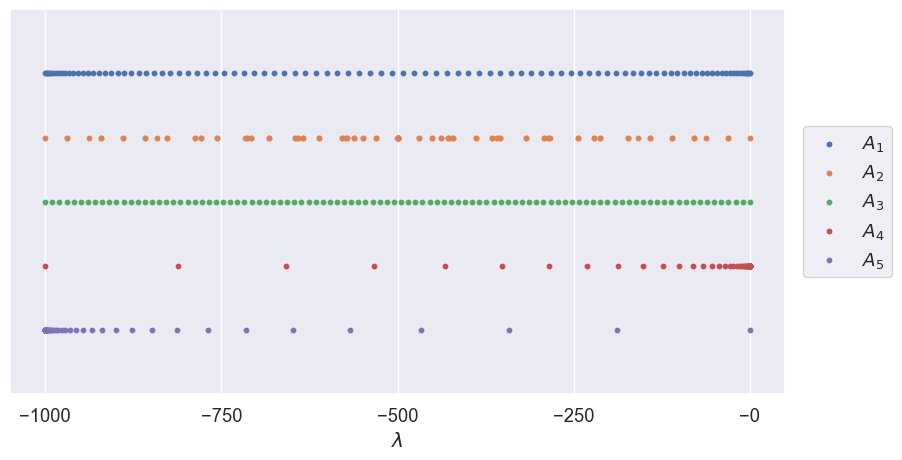
\includegraphics[width=.8\textwidth]{img/eigvals.png}
    \caption{
        Distribution of eigenvalues of the test matrices with $n=100$ and
        $\lambda = 1000$.
    }
    \label{fig:eigenvaluedistributions}
\end{figure}

\begin{comment}
    \begin{figure}[h]
        \centering
        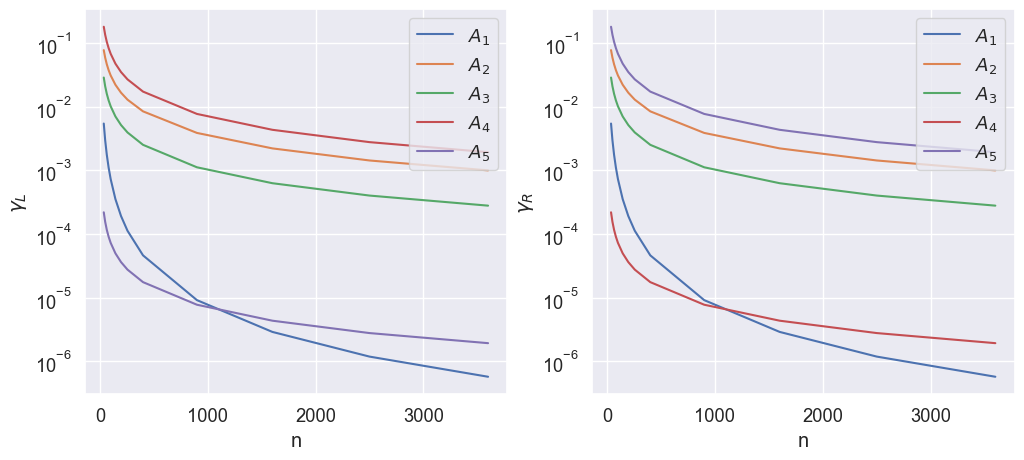
\includegraphics[width=.9\textwidth]{img/relgaps.png}
        \caption{
            Right and left relative gaps of the test matrices with
            $\lambda = 1000$ against their size.
            }
            \label{fig:relgaps}
        \end{figure}
\end{comment}

We are interested in evaluating $\varphi_p(-tA) v$ with $t \in \mathbb{R}$ being a time step.
We take $-\hat{A}_{1D} \in \mathbb{R}^{n \times n}$ and $-\hat{A}_{2D} \in \mathbb{R}^{n \times n}$
($n$ must have an integer square root), and we spectrally scale them so that they both have the
same spectral interval $[-\lambda, -\epsilon]$ with $\lambda > 0$ and $\epsilon = 0$.
We call the resulting matrices $A_1$ and $A_2$, respectively.
The spectral interval of a complex Hermitian or a real symmetric matrix is the smallest
interval in $\mathbb{R}$ that contains all the eigenvalues of the matrix, and it coincides
with the numerical range of the matrix.
Assuming that the spectral interval of the original matrix is $[\lambda_1, \lambda_n]$,
the spectral scaling is done by $A_i = -a \hat{A}_{iD} + b I$ for $i = 1, 2$; where the coefficients
are $a = (\lambda - \epsilon) / (\lambda_n - \lambda_1)$ and
$b = (\lambda \lambda_1 - \epsilon \lambda_n) / (\lambda_n - \lambda_1)$.
By scaling the matrices this way, we can focus on studying the effect of different eigenvalue
distributions on the same interval. The evaluation of $\varphi_p(-t\hat{A}_{iD}) v$ could then be
associated to $\varphi_p(A_i) v$ with $t \simeq \lambda / \lambda_n$ assuming that $\epsilon$
is sufficiently small and $\lim_{n \to \infty}\lambda_1 = 0$,
which happens to be the case for $\hat{A}_{1D}$ and $\hat{A}_{2D}$. For $\hat{A}_{1D}$ with
$n = 10^4$, for instance, picking $\lambda = 10^5$ corresponds to $t \simeq 2.5\mathrm{e}{-04}$.


Beside these two matrices, we consider three diagonal matrices of size
$n \times n$, $A_3$, $A_4$, and $A_5$, with eigenvalues distributed on the same
interval, $[-\lambda, -\epsilon]$. The eigenvalues of $A_3$ are distributed
uniformly. The eigenvalues of $A_4$ and $A_5$ are distributed geometrically so that
they are concentrated on right and left, respectively. We test with matrices with
different $\lambda$'s and different sizes.
\autoref{fig:eigenvaluedistributions} shows the eigenvalues of these matrices with
$n=100$ and $\lambda = 1000$.
\begin{comment}
An interesting property of these matrices could
be the relative distance between the two smallest and the two largest eigenvalues,
which we call left and right relative gap, respectively. More formally, if we
consider a $n \times n$ matrix $A$ with the eigenvalues
$\lambda_1 \le \lambda_2 \le \cdots \le \lambda_{n-1} \le \lambda_n$,
the left and the right relative gaps are
defined as
\begin{equation}
    \label{eq:relativegaps}
    \gamma_L = \frac{\lambda_2 - \lambda_1}{\lambda_n - \lambda_1}, \quad
    \gamma_R = \frac{\lambda_n - \lambda_{n-1}}{\lambda_n - \lambda_1}.
\end{equation}
These properties are illustrated for the test matrices in \autoref{fig:relgaps}.
Both relative gaps decrease for all the test matrices as the matrices grow in size.
For large $n$'s, $A_1$ always has the smallest relative gaps on both sides. $A_4$ and
$A_5$ always have the second place on right and left, respectively.
$A_2$ and $A_3$ have moderate relative gaps on both sides.
\end{comment}

% NOTE: Old table of test matrices
\begin{comment}
\begin{table}[h!]
    \centering
    \caption{
        Properties of the test matrices. The last column is the interval that includes the eigenvalues of the matrix,
        reported only if the matrix is Hermitian.
        }
    \label{tab:testmatrices}
    \begin{tabular}[h!]{|c||c|c|c|c|c|c|}
        \hline
        Name & Size & Density & Hermitian & \makecell{Full\\numerical\\rank} & \makecell{Condition\\number} & $\Omega \subset \mathbb{R}$ \\
        \hline
        \texttt{fd\_1d} & 4096 & 0.0007 & \checkmark & \checkmark & 6.80e+06 & $[-4, 0]$ \\
        \hline
        \texttt{fd\_2d} & 4096 & 0.0012 & \checkmark & \checkmark & 1.71e+03 & $[-8, 0]$ \\
        \hline
        \texttt{fd\_3d} & 4096 & 0.0012 & \checkmark & \checkmark & 1.16e+02 & $[-8, 0]$ \\
        \hline
        \texttt{orani678} & 2529 & 0.0141 & \texttimes & \checkmark & 9.58e+03 & - \\
        \hline
        \texttt{bcspwr10} & 5300 & 0.0008 & \checkmark & \texttimes & 1.58e+17 & $[-3, 7]$ \\
        \hline
        \texttt{gr\_30\_30} & 900 & 0.0096 & \checkmark & \checkmark & 1.95e+02 & $[0, 12]$ \\
        \hline
        \texttt{helm2d03} & 392257 & < 0.0001 & \checkmark & \checkmark & ? & $[0, 11]$ \\
        \hline
    \end{tabular}
\end{table}
\end{comment}

\subsubsection*{Pole Selection for Rational Krylov Approximation}

We use the \texttt{baryrat} library introduced in \cite{hofreither2021BRASIL} which implements
the AAA algorithm for rational approximations. One downside of using this algorithm
is the additional computational cost that it brings for computing the poles.
The AAA algorithm  computes the residual of the approximation on all the given interpolation points at
each iteration. Hence, for approximating a rational function of degree $m$, its computation cost scales
as $O(mn)$ where $n$ is the number of interpolation points given as input.
Furthermore, since this algorithm computes the poles based on the interpolation points, the
selected poles by this algorithm are very sensitive to the discretization of the interpolation domain.
Considering the $[-\lambda, 0] \subset \mathbb{R}$ interval, the number of interpolation
points for the AAA algorithm to work accurately scales with $\lambda$, which becomes a real burden
when $\lambda \to \infty$. However, as depicted in \autoref{fig:polesAAA}, numerical results show that
for this interval, the computed poles converge quite early when $\lambda$ is increased. We take
advantage of this behaviour and we pre-compute the poles by running the AAA algorithm
on the interval $[-10^{4}, -10^{-16}]$ with $30000$ logarithmically spaced interpolation points.
The poles for $\varphi_1$, $\varphi_3$, $\varphi_5$, and $\varphi_{10}$ are pre-computed and stored.
\todo[color=cyan]{Maybe some words regarding the choice of logarithmic distribution.}

Using the poles from this strategy, the maximum errors of the scalar rational approximations on different
intervals have been computed and are presented in \autoref{fig:errorsAAAms}. These plots show that
it is possible to reach a maximum error of $10^{-12}$ with a degree less than $15$.
On the other hand, it was observed that with degrees more than about $15$, the computed poles will take values
close to or on the negative real axis.
\autoref{fig:polesAAAms} illustrates this behavior for $\varphi_3$.
With $m=15$, we can see that some poles are getting close to the real negative axis. With $m=20$, 3 poles
lie on the negative real axis. With $m=25$, we can see that the situation is already very bad with many
poles lying on the negative real axis.
This could significantly impact the performance of the rational Krylov approximation method if the input
matrix has real negative eigenvalues, which happens to be the case for our test matrices.
Comparing the computed poles with different number of interpolation points in \autoref{fig:polesAAAms},
it can be concluded that when $m$ gets larger, more interpolation points are needed in order to compute
the poles accurately. This will justify the increased errors after $m=15$ for $\varphi_1$ in
\autoref{fig:errorsAAAms}.

For a rational Krylov subspace of dimension $m$, first take $k \le m$ pre-computed poles $\eta_1, \dots, \eta_k$
by the AAA algorithm and we repeat them enough times to fill the $m$ poles $\xi_1, \dots, \xi_m$.
With this scheme for the pole selection, the RA method is denoted by RA-AAAk where "k" is replaced
by its number.
We also consider the case with a single repeated pole $\xi_1 = \xi_2 = \cdots = \xi_{m} = 1$ and
we deonte it by RA-ONES.
When the poles are repeated, the LU decomposition of the matrix $I - A/\xi_j$ is computed
once for each pole and it is used for solving $w = (I - A/\xi_j)^{-1} A v_j$ in line 4 of
the modified version of \autoref{alg:polynomialarnoldi}.

\todo[color=gray]{
    Two other strategies have been considered but this one performs the best.
    1: Keeping the first m poles and repeating $\infty$ afterwards;
    2: Keeping the first m poles and repeating the last one afterwards.
}

\begin{remark}
    In order to approximate the scalar function, the AAA algorithm needs to evaluate the scalar
    $\varphi_p(z)$ many times in the interval.
    For $\varphi_0$ the scalar exponential is used. For $\varphi_1$, the \texttt{scipy.special.expm1}
    function divided by $z$ gives accurate evaluations for large and small $z$.
    For $\varphi_p$, $p > 1$, two methods are used depending on the absolute value of $z$.
    For $|z| > 1$, \eqref{eq:scalarphifunctionsrecurrence} is used in a recursive algorithm.
    However, for small $|z|$, this method lacks numerical stability because of multiple divisions by $z$.
    Hence, for non-zero $|z| < 1$, we use Corollary \ref{cor:embeddedmatrixexponential} and read $\varphi_p(z)$
    from the first entry of the last column of $\exp(\hat{A})$ with $\hat{A}$ being defined in
    \eqref{eq:embeddedmatrixdefinition} for the matrix-vector pair
    $(z \in \mathbb{C}^{1 \times 1}, 1 \in \mathbb{C}^{1})$.
    For $|z|$ smaller than machine precision, $\varphi_p(0) = \frac{1}{p!}$ is returned.
\end{remark}

\begin{figure}[h!]
    \centering
    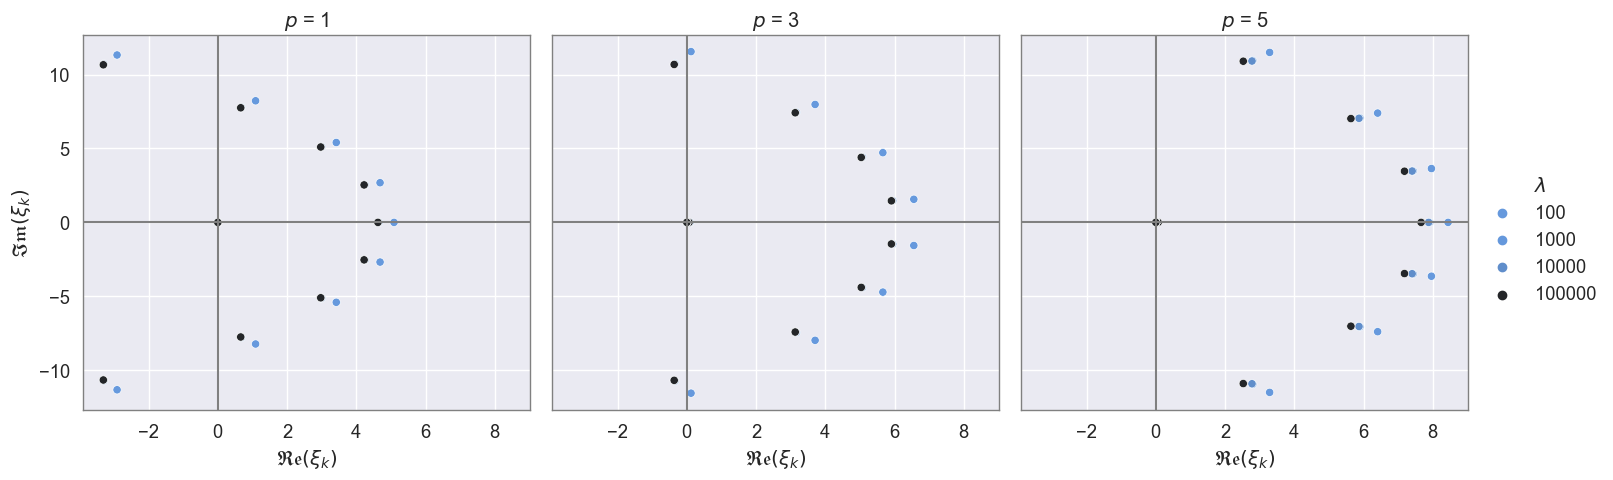
\includegraphics[width=.9\textwidth]{img/AAA/poles_lambda_log20k_m10.png}
    \caption{
        The first 10 poles computed by the AAA algorithm for $\varphi$-functions with $20000$
        logarithmically spaced interpolation points on the interval $[-\lambda, -10^{-16}]$.
    }
    \label{fig:polesAAA}
\end{figure}

\begin{figure}[h!]
    \centering
    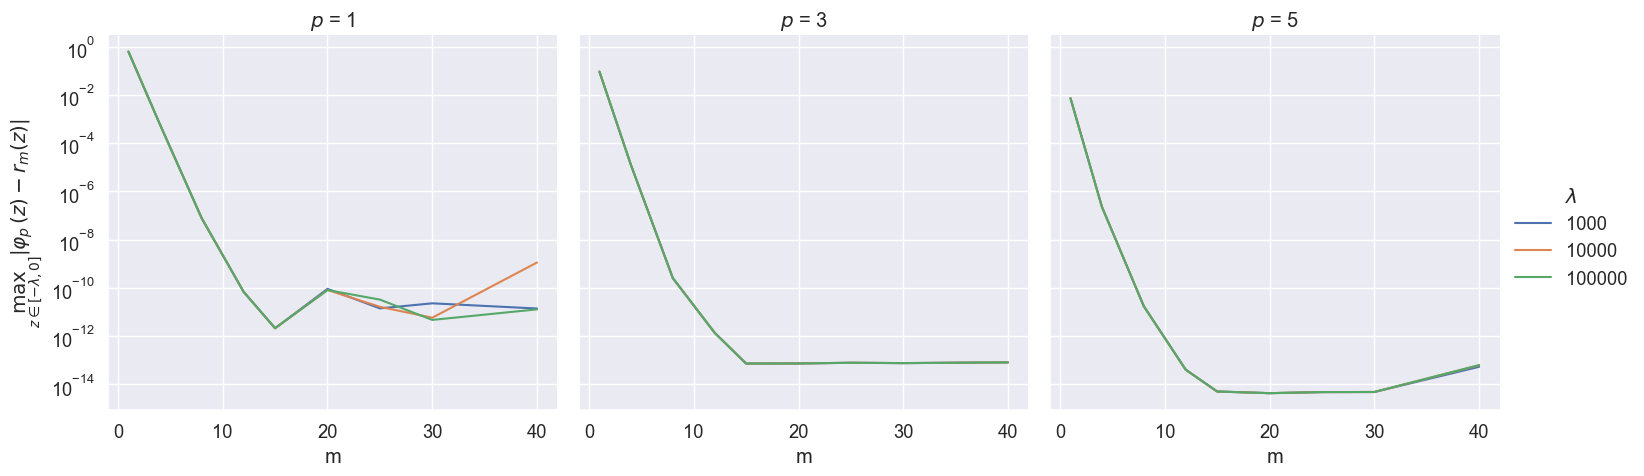
\includegraphics[width=.9\textwidth]{img/AAA/errors_ms_log30k.png}
    \caption{
        Maximum error of the rational approximation of $\varphi$-functions on the interval
        $[-\lambda, 0]$.
        The approximations are done on the interal $[-10^4, -10^{-16}]$ with $30000$
        logarithmically spaced interpolation points.
    }
    \label{fig:errorsAAAms}
\end{figure}

\begin{figure}[h!]
    \centering
    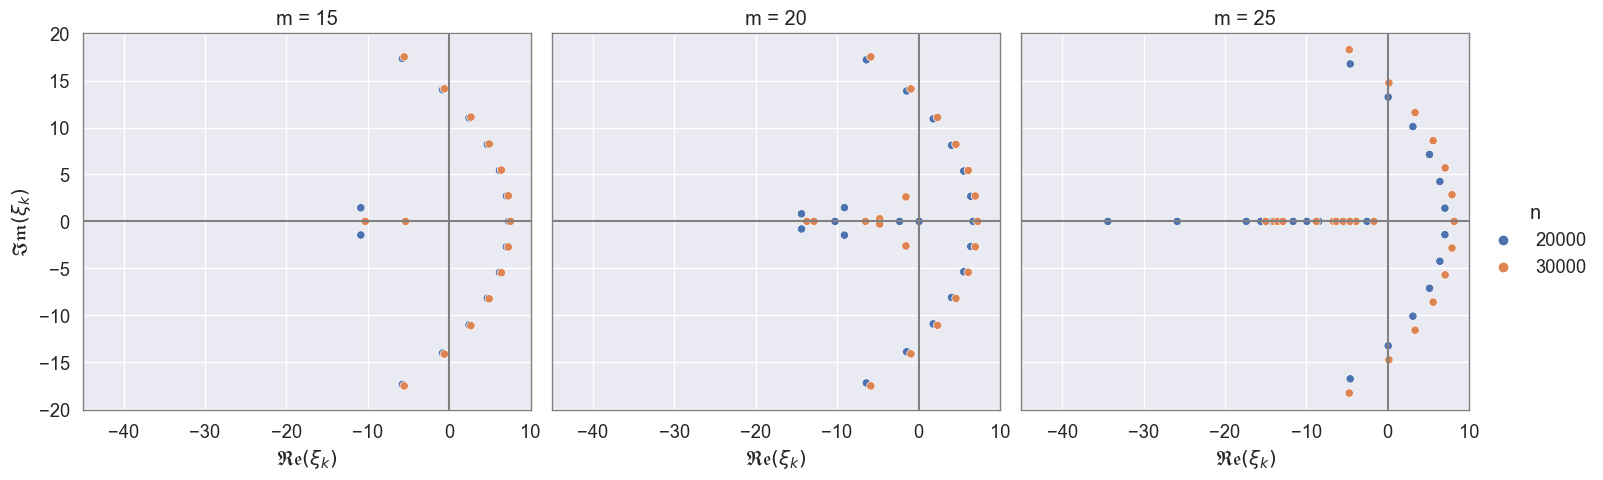
\includegraphics[width=.9\textwidth]{img/AAA/poles_ms_log_p03.png}
    \caption{
        Computed poles by the AAA algorithm for $\varphi_3$ with 20000 and 30000
        logarithmically spaced interpolation points on the interval $[-10^{4}, -10^{-16}]$.
    }
    \label{fig:polesAAAms}
\end{figure}


\subsubsection*{Numerical Results}
The methods described in \autoref{sec:polynomialkrylovapproximation} (PA)
and \autoref{sec:rationalkrylovapproximation} (RA)
are implemented and their approximations have been evaluated for the test matrices.
For all the test matrices, the approximations are carried out for a normalized
random vector $v$.
For computing $\exp(\hat{H}_m)$ and $\exp(\hat{A}_m)$, the \texttt{scipy.linalg.expm}
function from the the SciPy library~\cite{SciPy2020} is used which implements a Padé
approximation with a variable order that is decided based on the array data.
In order to evaluate the implementations, we take the vectors computed by the method
described in \autoref{sec:exactevaluation} as reference and we look at the relative
error of the results from the Krylov subspace methods of dimension $m$, denoted by
$\mathbf{\Phi_{p, m}}$, against the reference vectors, denoted by $\mathbf{\Phi_p^{EX}}$,
for different matrices. The relative error is computed as:
\begin{equation*}
    \delta_{rel}(\mathbf{\Phi_{p, m}}) =
    \frac{\left\| \mathbf{\Phi_{p, m}} - \mathbf{\Phi_p^{EX}} \right\|_2}
    {\left\| \mathbf{\Phi_p^{EX}} \right\|_2}.
\end{equation*}

\begin{figure}[h!]
    \centering
    \begin{subfigure}[b]{.9\textwidth}
        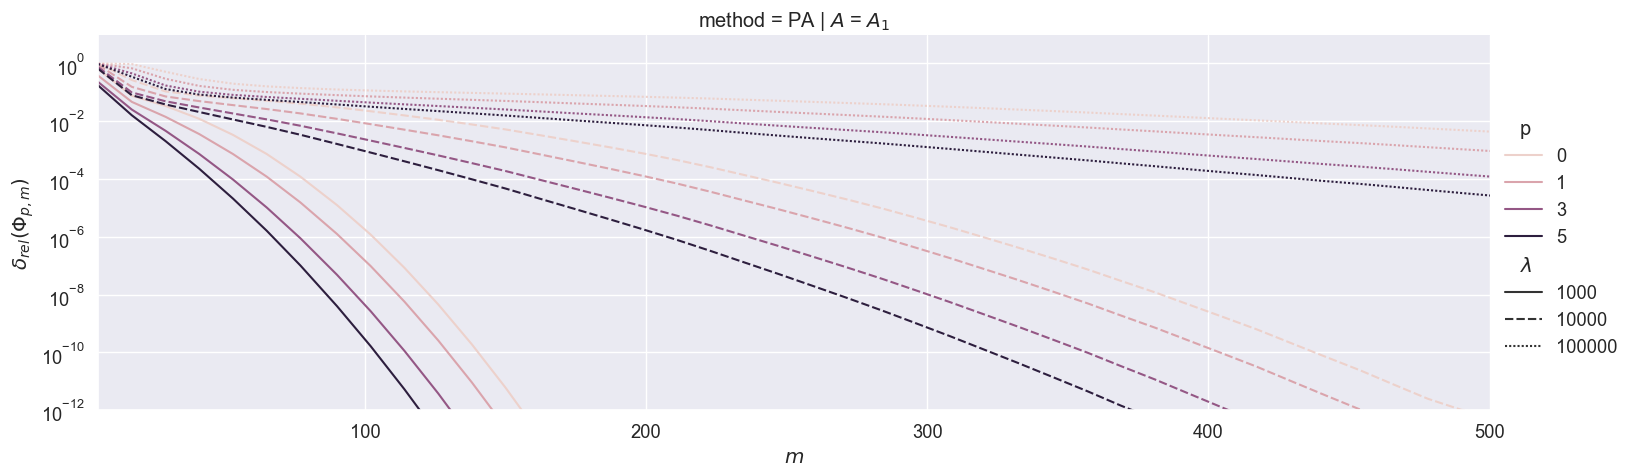
\includegraphics[width=\textwidth]{img/krylovapproximation/cnvg_ps_PA_n1e04.png}
        \caption{Polynomial Krylov approximation.}
        \label{fig:polynomialkrylovapproximationevaluation}
    \end{subfigure}
    \vfill
    \begin{subfigure}[b]{.9\textwidth}
        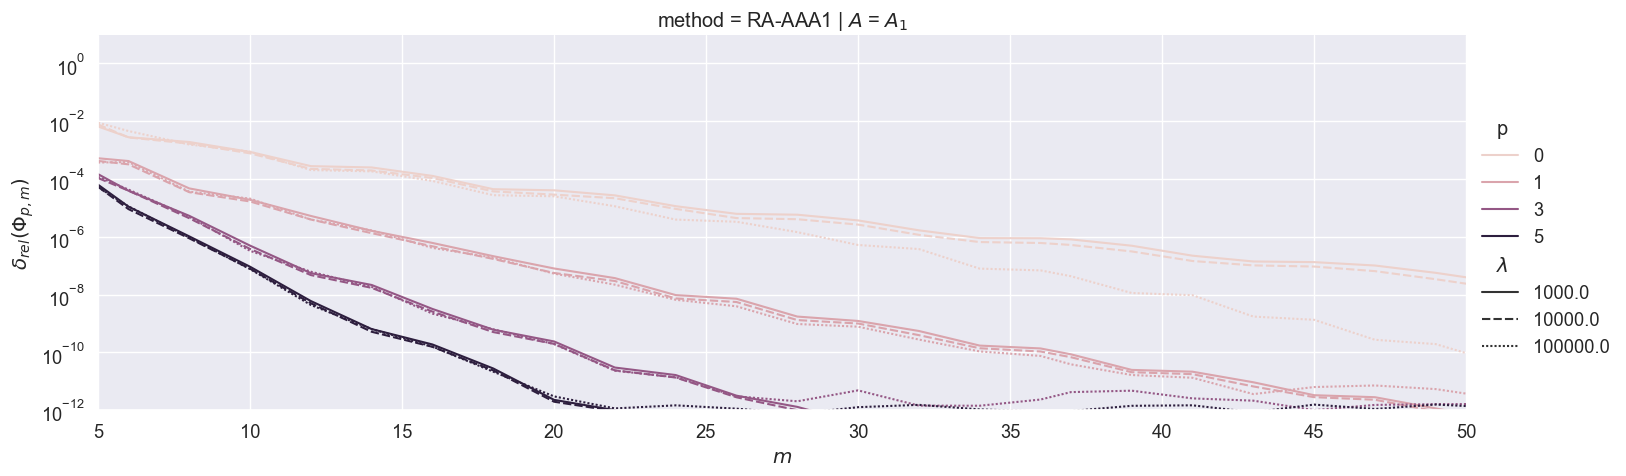
\includegraphics[width=\textwidth]{img/krylovapproximation/cnvg_ps_RA-AAA1_n1e04.png}
        \caption{Rational Krylov approximation.}
        \label{fig:rationalkrylovapproximationevaluation}
    \end{subfigure}
    \caption{
        Convergence of the approximations \eqref{eq:polynomialkrylovapproximation}
        and \eqref{eq:rationalkrylovapproximation} for matrices of size $n=10000$.
    }
    \label{fig:krylovapproximationevaluation}
\end{figure}

The convergence plots for the polynomial and the rational Krylov approximations are
illustrated in \autoref{fig:krylovapproximationevaluation} for $A_1$ with size $n=10000$.
We observe that both methods always converge slightly faster for larger $p$'s.
This observation is consistent with the error bound provided in Lemma
\ref{lem:univariateerrorestimationphitaylor}, where we can see that increasing $p$ slightly
improves the bound. This slight improvement could also be justified by looking at the
$\varphi$-functions on the complex plane. As depicted in
\autoref{fig:scalarphifunctionscomplexplane}, when $p$ is increased, the
function $\varphi_p$ grows more slowly on the real axis and thus it could be approximated
better with a polynomial of a fixed degree.
Therefore, the polynomial Krylov approximation needs less iterations to reach a certain tolerance according
to Theorem \ref{the:univariateerrorestimationgeneral}.
This hypothesis is also supported by \autoref{fig:errorsAAAmethods}.
As $\lambda$ goes to $\infty$, the convergence of the PA method deteriorates significantly.
On the other hand, the convergence of the RA method is not affected by the spectrum
of the matrix.

% CHECK:
% Comparing the convergence of the two matrices, we observe that even when the matrices have the
% same spectral interval, the convergence is much slower for $A_1$. This gives the notion that the distribution of
% the eigenvalues also plays an important role in the convergence of the method.

\todo{Update \autoref{fig:krylovapproximationcputime}.}
\todo{Update the comments about \autoref{fig:rationalkrylovpoleselection} and \autoref{fig:krylovapproximationcputime}.}

\begin{figure}[h]
    \centering
    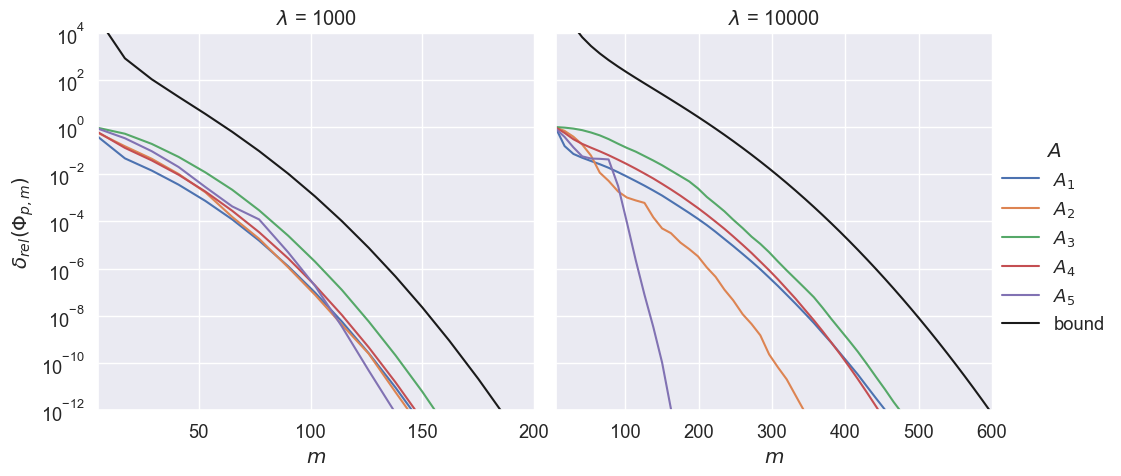
\includegraphics[width=\textwidth]{img/krylovapproximation/cnvg_matrices_PA_n10000.png}
    \caption{Convergence of the approximation \eqref{eq:polynomialkrylovapproximation}
    for $p=1$ with different test matrices of size $n=10000$ and the same spectral interval.
    The error estimation in \eqref{eq:univariateerrorestimationphi1} is plotted with black.}
    \label{fig:krylovapproximationmatrices}
\end{figure}

\begin{figure}[h]
    \centering
    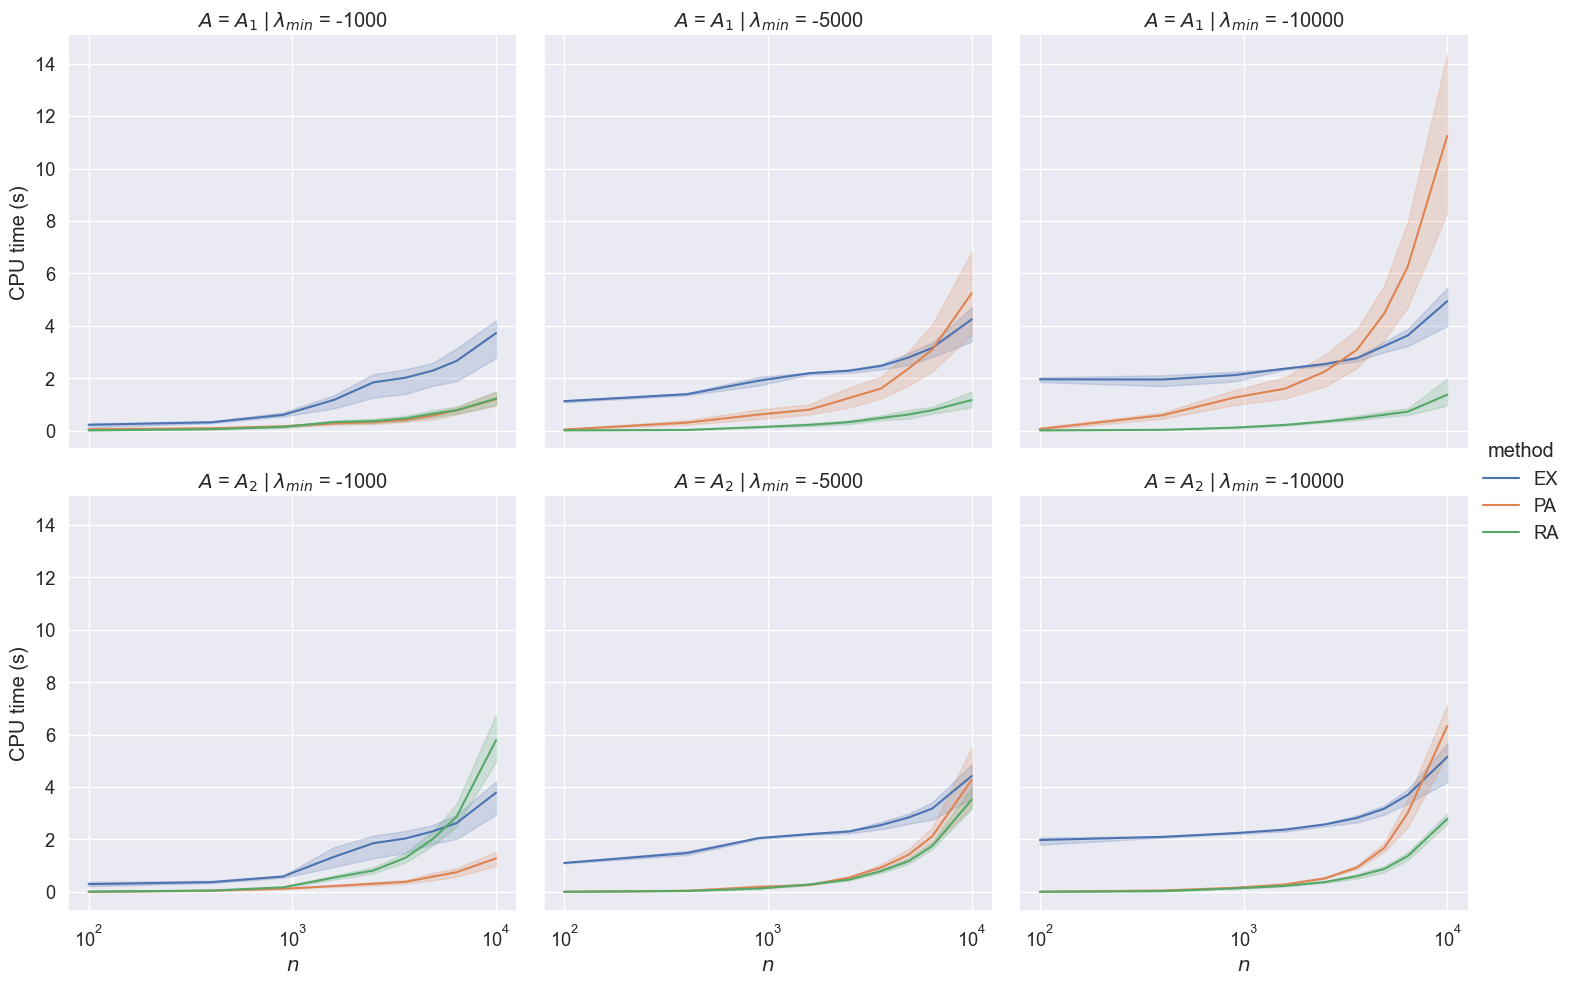
\includegraphics[width=.9\textwidth]{img/krylovapproximation/cputime_methods.png}
    \caption{
        CPU time for different evaluation methods. For the approximating methods,
        the minimum iterations required to reach a relative error less than $10^{-12}$
        is considered. Shadows of each line represent the range of the CPU time for
        $\varphi_0$, $\varphi_1$, $\varphi_3$, and $\varphi_5$.
    }
    \label{fig:krylovapproximationcputime}
\end{figure}

\autoref{fig:krylovapproximationmatrices} compares the convergence of the
test matrices with the same spectral interval, thus, the same smallest and largest
eigenvalues.
With $\lambda = 1000$, the method converges with almost the same rate for all
the test matrices, which is very close the same rate estimated in
\eqref{eq:univariateerrorestimationphi1}.
As $\lambda$ gets larger, we observe that the convergence for the matrices
$A_2$ and $A_5$ get considerably faster than the other matrices and the error estimate.
What these two matrices have in common is that the distributions of their eigenvalues
(see \autoref{fig:eigenvaluedistributions}) are less dense on the right side of their
spectral interval compared to the other test matrices.

In \autoref{fig:krylovapproximationcputime}, the process time of each method is presented for
the matrices $A_1$ and $A_2$ with different smallest eigenvalues against their sizes. For
the PA and RA methods, the reported process time corresponds to the minimum number of
iterations required by that method to reach a certain tolerance in its relative error.
For both matrices, the advantages of the RA method show themselves when the matrix gets
larger and the smallest eigenvalue is larger in magnitude. The PA method, on the other hand,
starts being less efficient than the reference solution when the smallest eigenvalue goes
to $-\infty$. The reason for this is that as mentioned before, the PA method needs more
and more iterations to converge when $\lambda \to \infty$.

\autoref{fig:rationalkrylovpoleselection} compares the convergence of the RA method with different
pole selection strategies. Repeating the first pole computed by the AAA algorithm already shows
advantages over repeating $\xi = 1$. As we increase the degree of the rational approximation by
the AAA algorithm, the convergence rates get higher but only until a certain degree.
The RA-AAA10 works the best among the presented pole selection strategies. It is noteworthy that
the rate of convergence with this method is higher when all the 10 poles are repeated equal times.
With the RA-AAAm strategy (approximating with rational function of degree $m+1$), the relative
error stagnates at around $10^{-8}$ and even before this error, the rate of convergence is close
to with only one repeated pole. This behaviour could be justified when we note that the poles
are obtained by approximating the function on an interval different than $[-\lambda, 0]$.
Increasing the degree of the rational approximant, thus, could worsen the approximation when the
whole interval is considered.

\begin{figure}[h]
    \centering
    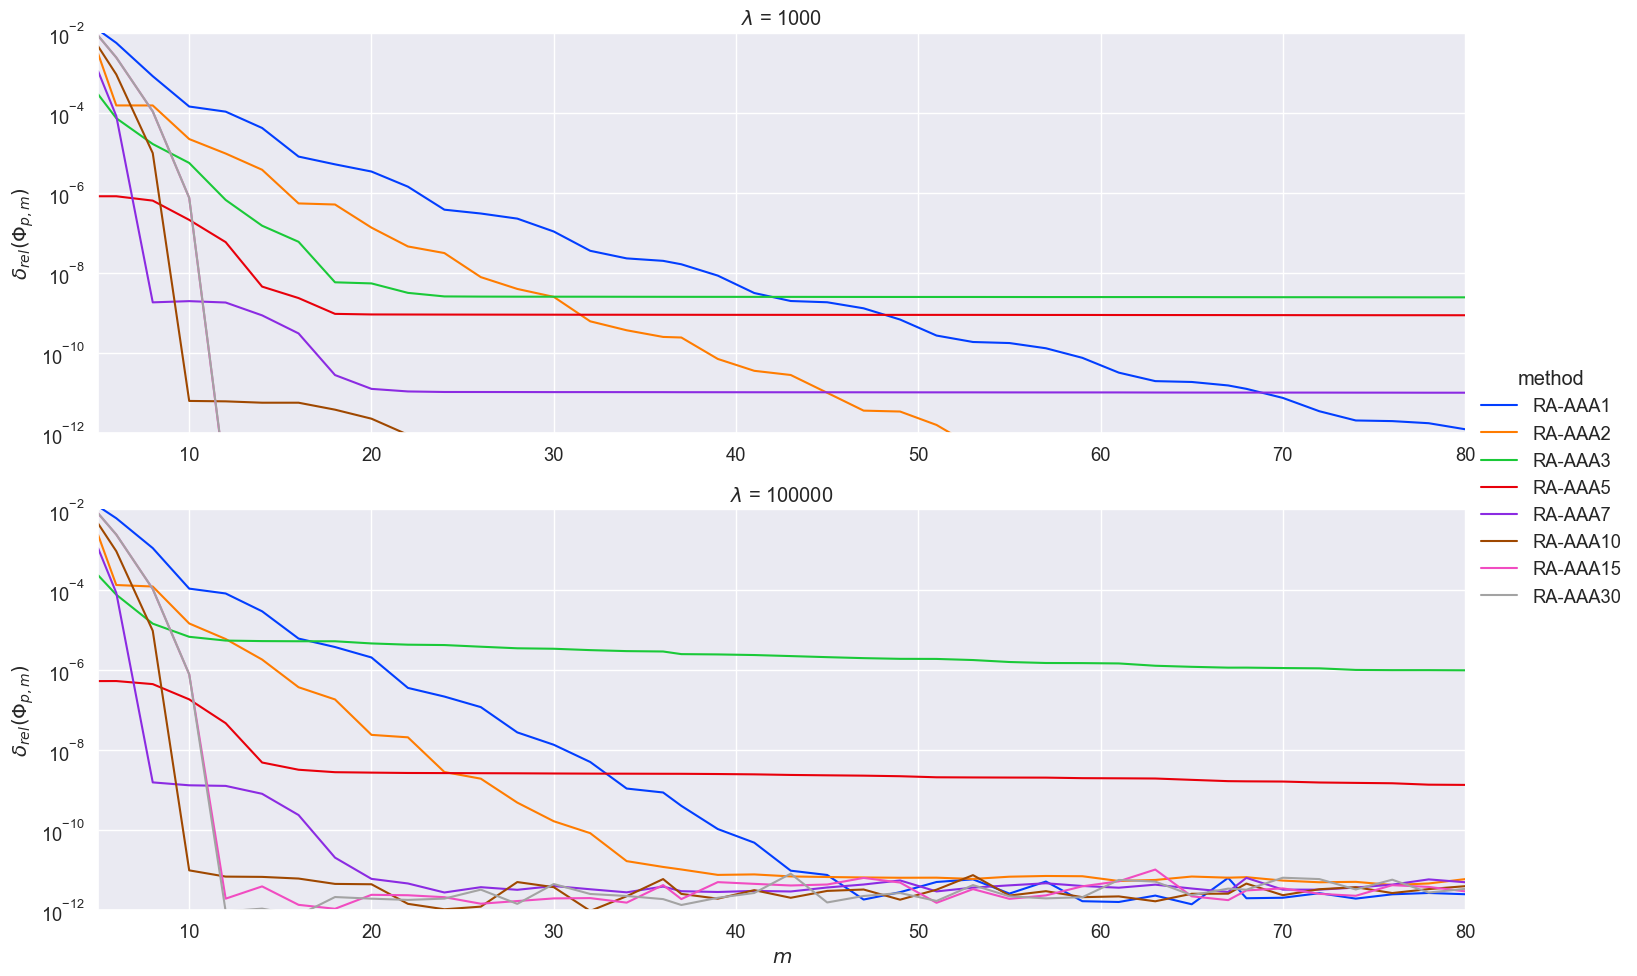
\includegraphics[width=.9\textwidth]{img/krylovapproximation/cnvg_poles_n1e04_p03.png}
    \caption{
        Convergence of the approximation \eqref{eq:rationalkrylovapproximation} with different
        pole selection strategies for $A_1$, $p=3$, and $n=10^4$.
    }
    \label{fig:rationalkrylovpoleselection}
\end{figure}

\FloatBarrier
\subsection{Trigonometric Matrix Functions}
\todo{Describe the context and linear elasticity.}
\subsubsection*{Test Matrices}
\todo{Describe the linear elasticity matrices.}
\subsubsection*{Pole Selection}
\todo{Describe the pole selection and the reason behind it.}
\todo[color=gray]{
    AAAn performs the best with n=1.
}
\todo[color=gray]{
    I use 1000 points on the spectral interval of the input matrix.
}
\subsubsection*{Numerical Results}
\todo{Comment on the figures.}

\begin{figure}[h]
    \centering
    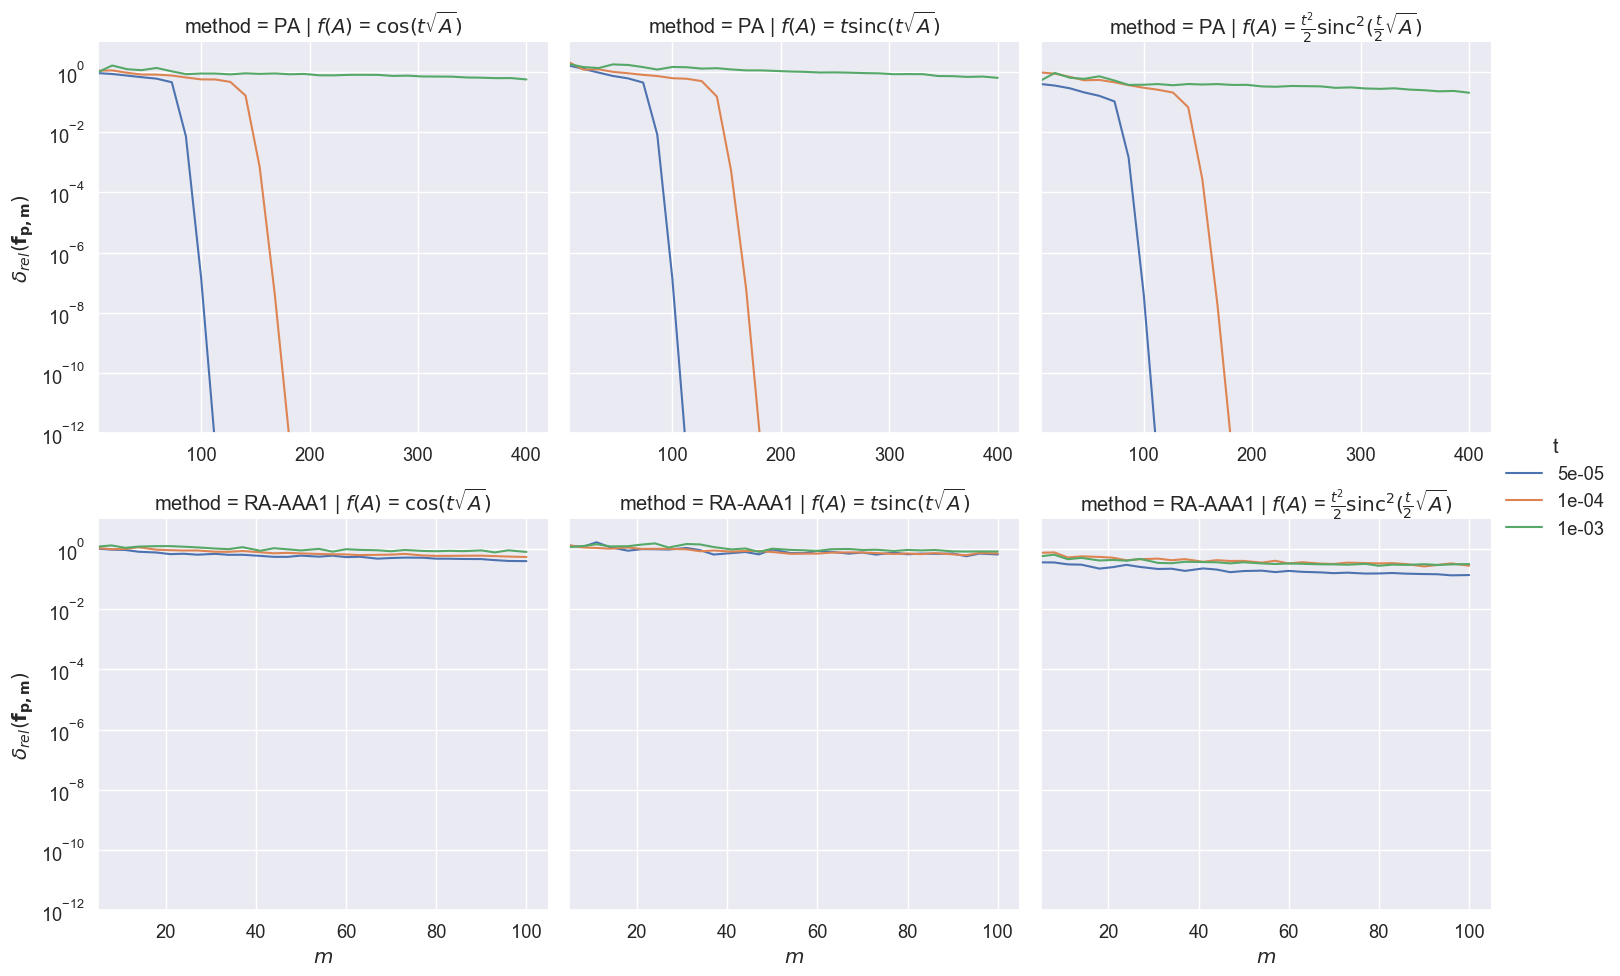
\includegraphics[width=.9\textwidth]{img/trigonometric/cnvg_h4e-02_methods_PA:RA.png}
    \caption{
        Convergence of the approximations \eqref{eq:polynomialkrylovapproximation}
        and \eqref{eq:rationalkrylovapproximation} with time steps for $A_{LE}^{h=0.04}$.
        }
        \label{fig:trigonometricconvergencetimesteps}
\end{figure}

\begin{figure}[h]
        \centering
        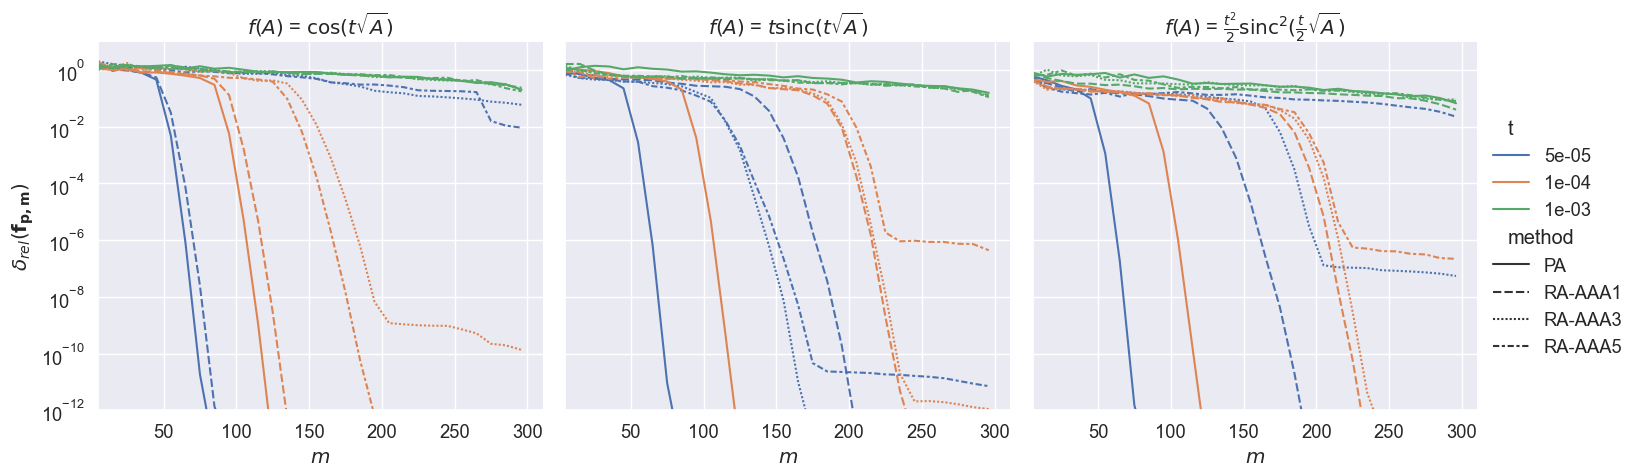
\includegraphics[width=.9\textwidth]{img/trigonometric/cnvg_h7e-02_methods.png}
        \caption{
            Convergence of the approximations \eqref{eq:polynomialkrylovapproximation}
            and \eqref{eq:rationalkrylovapproximation} with different
            rational function approximation methods for $A_{LE}^{h=0.07}$.
        }
        \label{fig:trigonometricconvergencemethods}
\end{figure}

\section{Conclusion}
\label{sec:conclusion}

% Cite Trefethen (Approximation Theory, p278):
% Polynomials cannot do the job at all for exp(x) in [-\infty, 0]!!
